\documentclass[12pt]{extarticle}
\usepackage[utf8]{inputenc}
\usepackage{amsmath}
\usepackage{cite}
\usepackage{hyperref}
\usepackage{graphicx}
\usepackage{caption}
\usepackage{subcaption}

\title{Mining latent relationships in stocks daily movements}
\author{Data Science For Networks: project report\\\\Giuseppe Attanasio\\ S265910}
\date{\today}

\begin{document}

\maketitle
\newpage

\section{Introduction}

Stock trading is an interesting applicative field where a significant number of machine learning and pattern recognition solutions are being designed to support traders decisions. Financial markets have become a breeding ground both for the availability of large and heterogeneous data sets and for the presence of several underlying economical rules that drive the market that can be mined. 

This work aimed to analyze relationships between price movements of different stocks in order to find similar \textit{behaviors}. The study focused on unsupervised modeling of stock prices variations by means of a multi-way representation. A tensor decomposition algorithm was applied to spot relevant information. 

\subsection{Modeling price variations}

The strategy for data modeling is a crucial and discriminant factor in this type of analysis. Since a tensor decomposition algorithm is used, the number and type of dimensions as well as the content of the cells has to be chosen.
The solution proposed is based on a graph-based representation built with the following steps.

\begin{enumerate}
    \item Since price data comes with a daily frequency, it is possible to compute the Rate Of Change (ROC) of closing prices with respect to the previous day: 
    \begin{equation}
        ROC_t = 100 \cdot \frac{C_t - C_{t-1}}{C_{t-1}}
    \end{equation}
    \item Then, each day is labeled using its ROC value and a threshold \textit{tr}:
    $$
        L_t = 
    	\begin{cases}
    		UP, & \text{if } ROC_t > tr \\
    		MID, & \text{if } -tr \leq ROC_t \leq tr \\
    		DOWN, & \text{if } ROC_t < -tr
    	\end{cases}
    $$
    \item Once days are labeled for each stock, build a graph $G = (V,E)$ where each vertex represents a stock and edges are created, for a given day \textit{t}, if both the stocks had a positive variation:
    \begin{equation}
        \forall i,j: L_{t,i} = UP \wedge L_{t,j} = UP \Rightarrow \exists e(i,j)
    \end{equation}
\end{enumerate}

Given this representation, each day, price relationships that were raising up can be depicted as a undirected graph, synthesized by a symmetric adjacency matrix with binary values in cells. 
Furthermore, the graph is not static. It changes day-by-day accordingly to updated information. Consequently, all the information may be encoded in a third-order tensor having the stocks on two axis and the time along the third:
$$
    X \in {\rm I\!N}^{S x S x T}
$$
Any slice of the tensor at time \textit{t} represents the adjacency matrix for the day \textit{t}. Additionally, the tensor is partially symmetric because all its slices along \textit{t} axis are symmetric.

\subsection{Tensor decomposition}

In this work the CANDECOMP/PARAFAC (CP) \cite{carroll1970analysis}\cite{harshman1970foundations} tensor decomposition was used to spot latent factors that generated the tensor - the reader here should read: \textit{the factors characterized by certain stocks that have grown together across the time}. 
There exist many matrix decomposition techniques used in collaborative filtering and recommendation tasks. CP factorization can be seen as a higher-order decomposition with respect to, for example, Singular Value Decomposition. 
The factorization generates an approximation of the original third-order tensor, expressed as a sum of \textit{R} rank-one tensors.
$$
    \hat{X} = \sum_{r=1}^R a_r \circ b_r \circ c_r
$$
while the single cell:
$$
    \hat{x}_{ijk} = \sum_{r=1}^R a_{ir} b_{jr} c_{kr}
$$

The latent factors can be spotted on components generated by the decomposition. As pointed out by Papalexakis \cite{papalexakis2016automatic}, each component highlights a soft co-clustering of the tensor, with the high values of $$ a_r, b_r, c_r $$ as the membership values to co-clusters.    

\section{Case study: S\&P500 stocks in 2017}

Even though there exist many stock market indices, the analysis is narrowed to Standard and Poor 500 index. It gathers the top 500 influential companies in United States of America. The temporal window analyzed is the solar year 2017.
The shape of the third-order tensor would be in principle
$
	500 x 500 x 365
$.
Considering only those stocks whose Global Industry Classification Standard (GICS) sector is known and the business days when the market was open, the input tensor become:
$$
	X \in {\rm I\!N}^{496 x 496 x 250}
$$

In order to encode only strong relationships, a threshold value of $ 2 \% $ was used. In financial market context this value is way higher than the common variation range [-1\%, 1\%] that stock prices unlikely cross.  

\subsection{Sparsity and connected components}

The choices for building the graph corresponding to one time step lead to a very sparse distribution as well as an high number of connected components. As an example, several adjacency matrices are reported in Figure \ref{fig:adj_matrices}.

\begin{figure}[!h]
	\centering
	\begin{subfigure}{0.48\textwidth} % width of left subfigure
		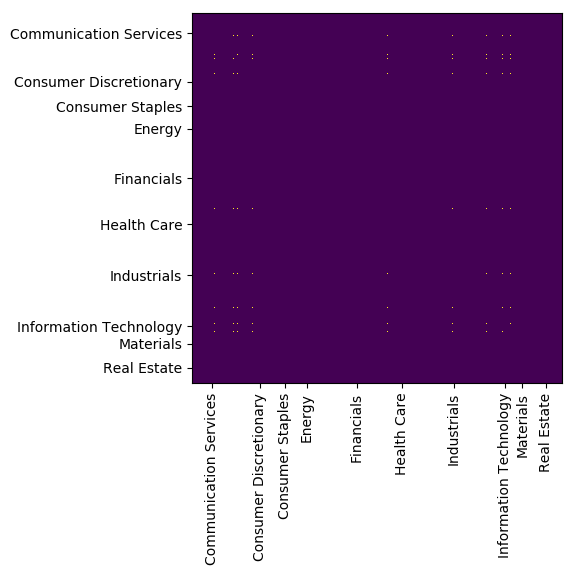
\includegraphics[width=\textwidth]{adj_50.png}
		\caption{Sample at 20 \% of the year} % subcaption
	\end{subfigure}
	\vspace{1em} % here you can insert horizontal or vertical space
	\begin{subfigure}{0.48\textwidth} % width of right subfigure
		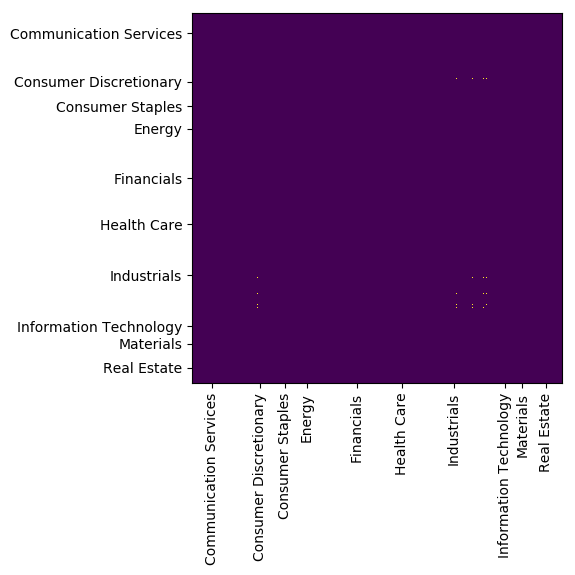
\includegraphics[width=\textwidth]{adj_100.png}
		\caption{Sample at 40 \% of the year} % subcaption
	\end{subfigure}
	\begin{subfigure}{0.48\textwidth} % width of right subfigure
		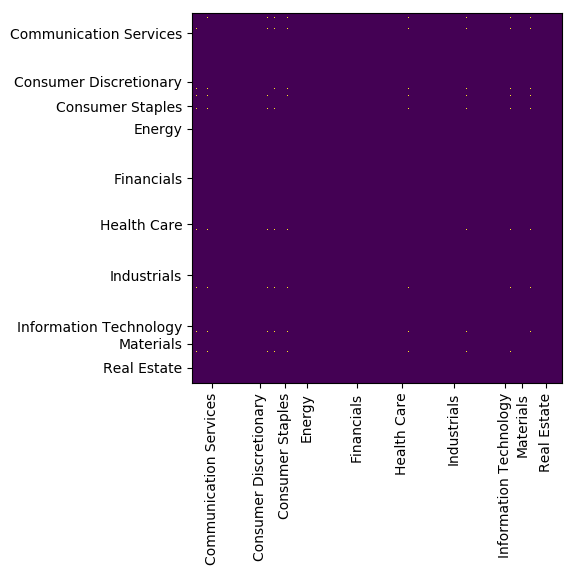
\includegraphics[width=\textwidth]{adj_150.png}
		\caption{Sample at 60 \% of the year} % subcaption
	\end{subfigure}
	\begin{subfigure}{0.48\textwidth} % width of right subfigure
		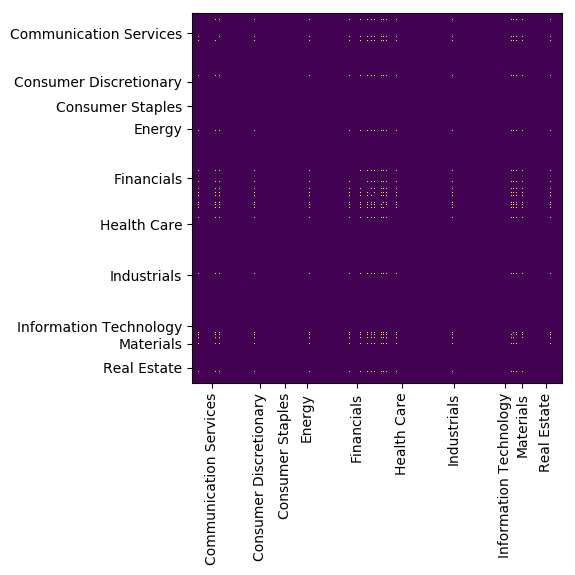
\includegraphics[width=\textwidth]{adj_200.png}
		\caption{Sample at 80 \% of the year} % subcaption
	\end{subfigure}
	\caption{Adjacency matrix for sample days} % caption for whole figure
	\label{fig:adj_matrices}
\end{figure}

Every stock-node whose growth was higher than the threshold is connected with all other stocks that behaved equally. As a consequence, every \textit{daily} graph is characterized by many unconnected nodes and one single fully connected component.
Even though it is difficult to display a visual representation of a graph with such a large number of edges and nodes, those peculiarities become clear analyzing connected components. The latter are reported in Figure \ref{fig:cc_by_time} and \ref{fig:cc_distribution}.

\begin{figure}[!h]
	\centering
	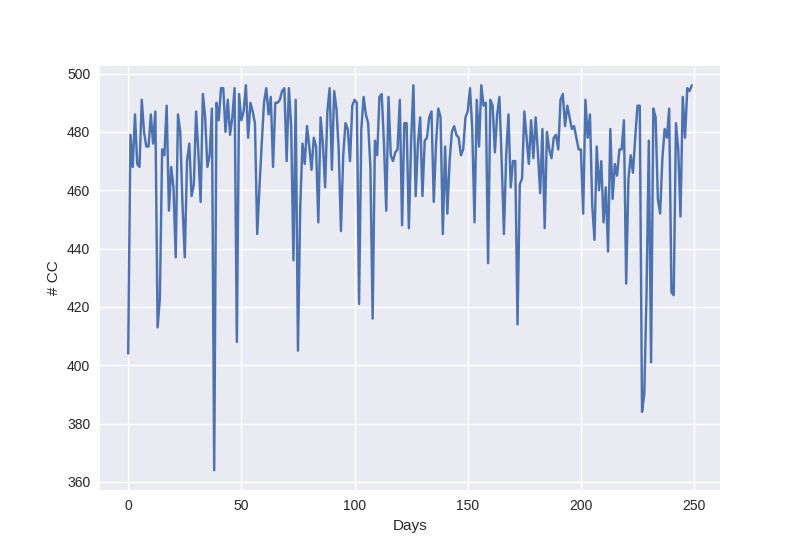
\includegraphics[width=0.8\textwidth]{cc_by_time.png}
	\caption{Number of connected components each day of the year. The larger the value on y-axis the larger the number of unconnected nodes - i.e. the lower the number of stocks that, on that day, have grown together.} 
	\label{fig:cc_by_time}
\end{figure}

\begin{figure}[!h]
	\centering
	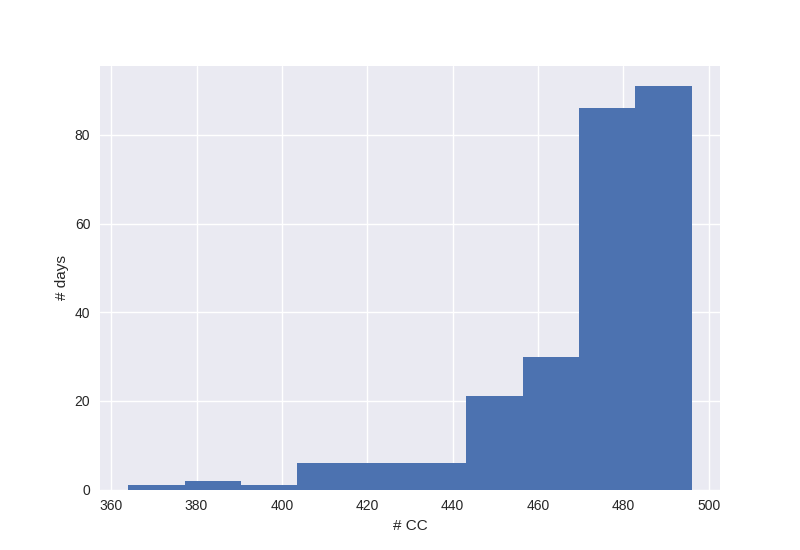
\includegraphics[width=0.8\textwidth]{cc_distribution.png}
	\caption{The distribution of connected components considering their number each day of the year.} 
	\label{fig:cc_distribution}
\end{figure}

\subsection{Latent factor analysis}

The analysis of latent factor is possible thanks to CP decomposition. The main parameter for the algorithm is \textit{R}, the number of components the sum of which approximates the original third-order tensor. The choice of the right \textit{R} is known to be a complex task, especially for very sparse tensor and for binary cell values - e.g. in \cite{papalexakis2016automatic}, \textit{AUTOTEN} includes an automatic quality assessment for the decomposition.\\
In this work, \textit{R} was chosen analyzing the error defined as the squared Frobenius norm of the difference between the real tensor and its reconstruction:
$$
	E = || X - \hat{X} ||^2_F
$$

Figure \ref{fig:errors_trend_line} shows that the resultant chart is not \textit{elbow-shaped} as expected. Since it was not possible to assess that after a given \textit{R} the error decay becomes less significant, another strategy was used.

\begin{figure}[h]
	\centering
	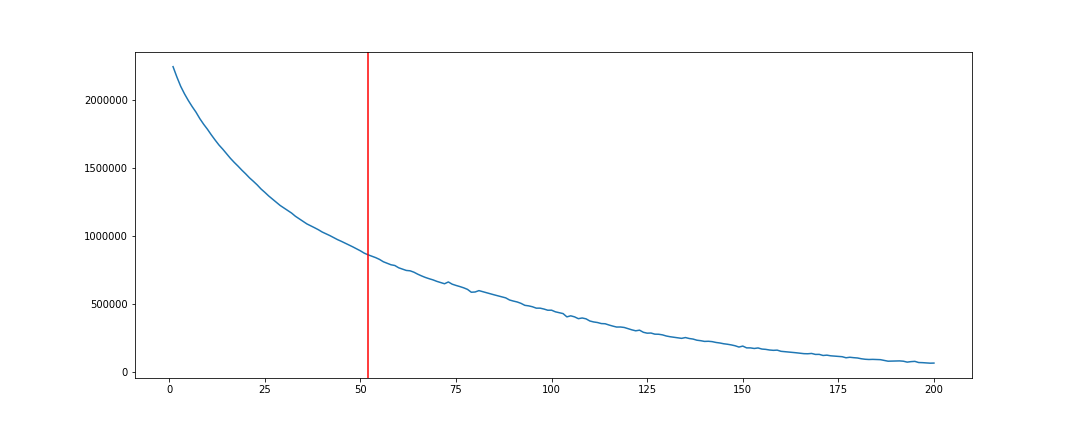
\includegraphics[width=\textwidth]{errors_trend_line.png}
	\caption{The reconstruction error versus the number of components. The orange line highlights the choice $ R = 52 $.} 
	\label{fig:errors_trend_line}
\end{figure}

The value $ R = 52 $ was chosen by evaluating an approximation of the discrete second derivative with explicit Euler's formula:
$$
	d(E)_t = E_{t-1} + E_{t+1} - 2 E_t
$$
and picking the point with maximum value. That value corresponds to point of the curve with maximum concavity.\\ 

Given this choice of R, 52 latent factors were produced. Each component is characterized by three column vectors:
\begin{itemize}
	\item $S_1^{(500x1)}$: \textit{weights} of stocks relative to that factor;
	\item $S_2^{(500x1)}$: \textit{weights} of stocks relative to that factor;
	\item $T^{(250x1)}$: \textit{weights} of time steps relative to that factor.
\end{itemize}
For sake of simplicity, this report includes only a subset of the 52 factors - in Appendix section it is reported a link to the Jupyter Notebook of the project containing the other charts. Furthermore, since there are almost 500 stocks, for synthesis purposes, factor plots were created by:
\begin{enumerate}
	\item ranking by value in descending order the stock weights;
	\item retaining only the top 5\%;
	\item grouping by GICS sector the weights. 
\end{enumerate}

All factors have a temporal component characterized by spikes in short periods of one or two days across the year. It could be a consequence of the binary encoding: the main membership stocks of the factor have a simultaneous growth in a restricted period while they are not related the rest of the time.\\
Co-clusters are not always clear since $S_1$ and $S_2$ contains similar rankings of the stocks (with a different scale): it is clear in Figure \ref{fig:f26}.

\begin{figure}[h]
	\centering
	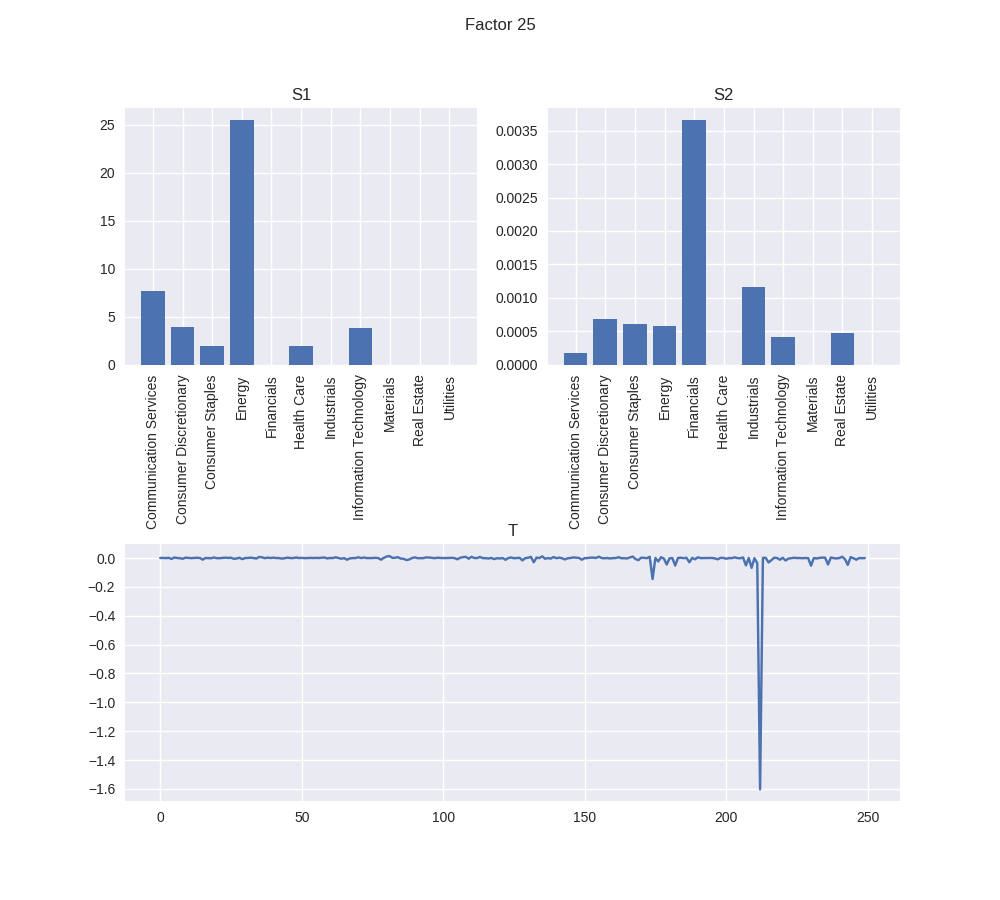
\includegraphics[width=\textwidth]{factor_25.png}
	\caption{Factor 25.} 
	\label{fig:f25}
\end{figure}

Figure \ref{fig:f25} instead shows two clear dominant sectors: \textit{Energy} and \textit{Financials}. Such result might suggest that stocks belonging to those sectors have had similar periods of growth. 

\begin{figure}[h]
	\centering
	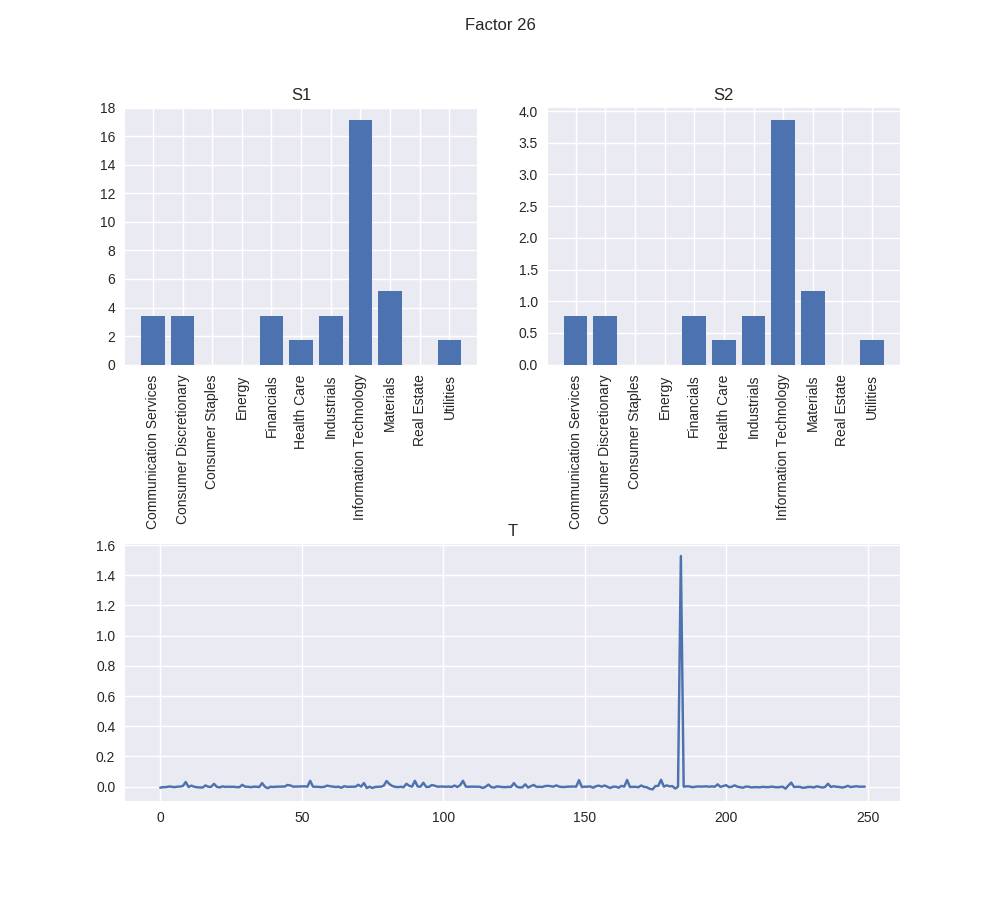
\includegraphics[width=\textwidth]{factor_26.png}
	\caption{Factor 26.} 
	\label{fig:f26}
\end{figure}

Figure \ref{fig:f40} reports two quite different distributions in $S_1$ and $S_2$. The most influential sectors are not overlapped: \textit{Industrials} and \textit{Information Technology} lead in $S_1$ and \textit{Communication Services}, \textit{Consumer Discretionary}, \textit{Consumer Staples} and \textit{Materials} lead in $S_2$.

\begin{figure}[h]
	\centering
	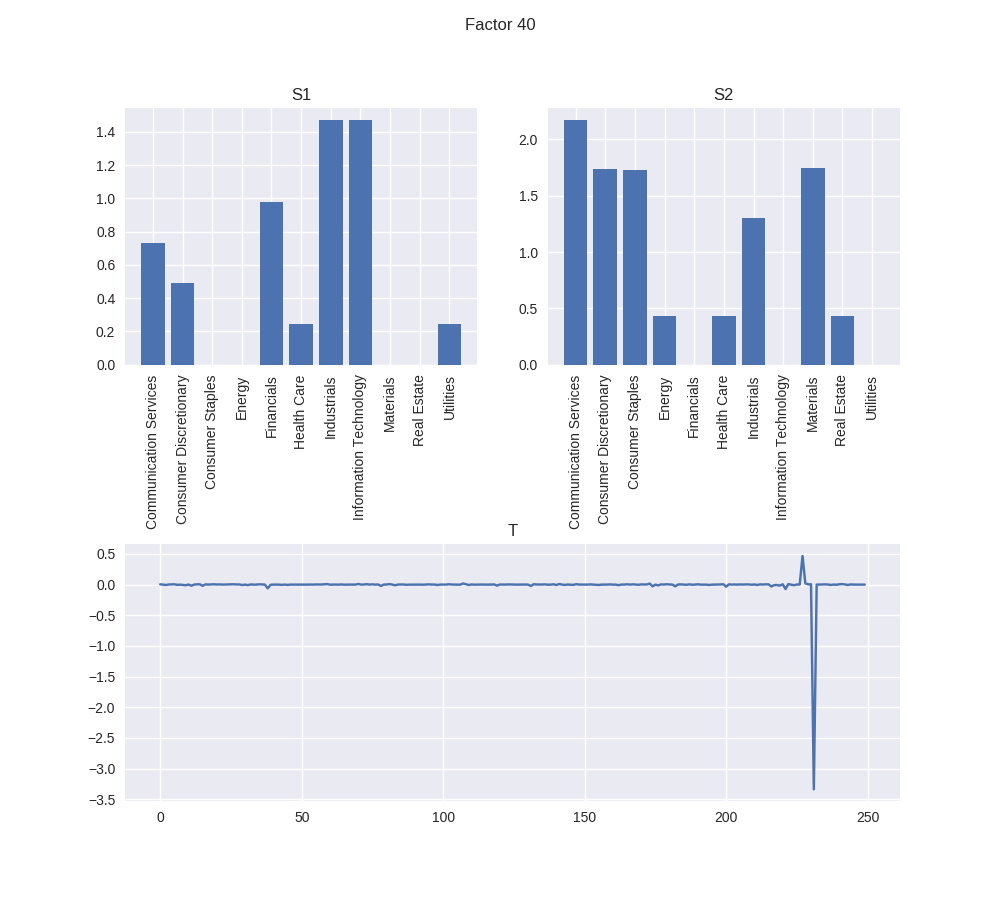
\includegraphics[width=0.99\textwidth]{factor_40.png}
	\caption{Factor 40.} 
	\label{fig:f40}
\end{figure}

\section{Conclusion and future works}

This work aimed to highlight underlying relationships in stock price movements. What is known and consolidated is that stocks of the same sectors are likely going to move together across the time: they are likely influenced by the same external factors. The results highlighted in most of the cases that this rule is true: many latent factors have shown the highest values for stocks belonging to the same sector.\\
Nevertheless, the most interesting results regard those latent factors where membership values are not stocks within the same sector. They potentially give valuable information on positively correlated stocks.\\
Surely this work requires deeper exploration of several aspects. $S_1$ and $S_2$ appear to have similar distribution in most cases. It might be a bias introduced by the partially symmetric representation of input tensor - it recalls \textit{SVD} decomposition of a positive symmetric matrix that generates two identical orthonormal factors. Given that, it could be useful explore a different encoding for tensor cells - e.g. using continuous values as the difference between the growth of the stocks. Another possibility would be a temporal aggregation: it would be equivalent to sum up two or more adjacency matrices and, consequently, eventually generate tensor cells larger than 1.\\
Finally, since the CP decomposition could not fit well with sparse binary tensors, this work could have an interesting extension with Boolean Tensors Decomposition. Unfortunately, such technique has not a ready-to-use implementation yet.

\section{Appendix}

The code and the complete list of results are available at:\\ \href{https://github.com/g8a9/dsnet}{https://github.com/g8a9/dsnet}\\
The Jupyter notebook used for the project is available at:\\
\href{https://github.com/g8a9/dsnet/blob/master/final_project.ipynb}{https://github.com/g8a9/dsnet/blob/master/final\_project.ipynb}

\bibliographystyle{plain}
\bibliography{M335}

\end{document}